\documentclass[border=10pt]{standalone}
\usepackage{pgfplots}
\pgfplotsset{width=7cm,compat=1.8}
\begin{document}
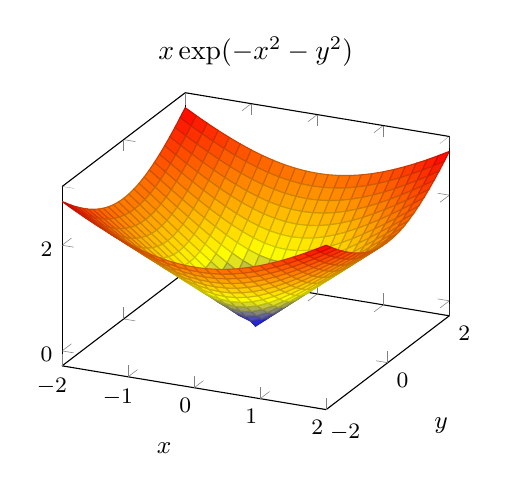
\begin{tikzpicture}
\begin{axis}[
    title={$x \exp(-x^2-y^2)$}, 
    xlabel=$x$, ylabel=$y$,
	small,
]
\addplot3[
	surf,
	domain=-2:2,
	domain y=-2:2,
] 
	{sqrt(x^2 + y^2)};

\end{axis}
\end{tikzpicture}
\end{document}


